%---------- Quinto Capítulo: Desenvolvimento do Software ----------
\chapter{Desenvolvimento do Software}
\label{chap:desenv}

Utilizando a metodologia e o projeto do sistema apresentados nos capítulos \ref{metod} e \ref{specs}, respectivamente, inicou-se o desenvolvimento efetivo do sistema.
Primeiramente foi criado um projeto Maven principal denominado \texttt{onibuscerto}, o qual foi dividido em quatro subprojetos: 
\begin{itemize}
	\item \texttt{onibuscerto-api}: contém a classe que representa coordenadas geográficas e o objeto resposta contendo informações da rota ao Cliente.
	\item \texttt{onibuscerto-core}: consiste no módulo \emph{Core} definido no projeto do software (seção \ref{specs}). 
	Contém as representações das entidades originárias dos arquivos GTFS e faz interface do sistema com o banco de dados.
	\item \texttt{onibuscerto-importer}: consiste no módulo \emph{Importer} definido no projeto do software (seção \ref{specs}).
	Responsável pela importação dos dados contidos nos arquivos GTFS para o sistema através das funcionalidades do \emph{Core}.
	\item \texttt{onibuscerto-service}: consiste nos módulos \emph{Web Service} e Cliente definidos na seção \ref{specs}. 
	Pretende-se futuramente separar este subprojeto em dois outros distintos representando tais módulos.
\end{itemize}

Nas subseções a seguir serão descritos detalhes a respeito da implementação de cada subprojeto.

\section{Configuração do ambiente de desenvolvimento}

\section{onibuscerto-core}

O \emph{Core} consiste basicamente na interface do sistema com o banco de dados, contendo portanto as representações das entidades originárias dos arquivos GTFS.
Estas representações nada mais são do que \emph{wrappers}, ou seja, classes no sistema que são responsáveis pelo encapsulamento das entidades do banco de dados.
Cada uma destas classes é implementação de uma respectiva interface, e tem o intuito de referenciar um nó ou aresta do grafo armazenado.

O \emph{Core} foi organizado de tal forma que todas as suas classes de entidades possuam suas respectivas \emph{factories}.
Como já comentado, \emph{factory} consiste em uma interface com o objetivo de criação de famílias de objetos dependentes ou correlacionados.
Desta forma, toda criação de entidades é realizada através de uma \emph{factory}, centralizando este processo a somente uma classe por entidade.

Cada \emph{factory} de entidade pertencente ao arquivo GTFS é armazenada no banco de dados como um nó de referência, o qual possui uma relação para cada nó de sua respectiva entidade.
Esta organização das \emph{factories} no grafo pode ser observada na figura \ref{fig:grafoFactory}.

\begin{figure}[!htb]
	\centering
	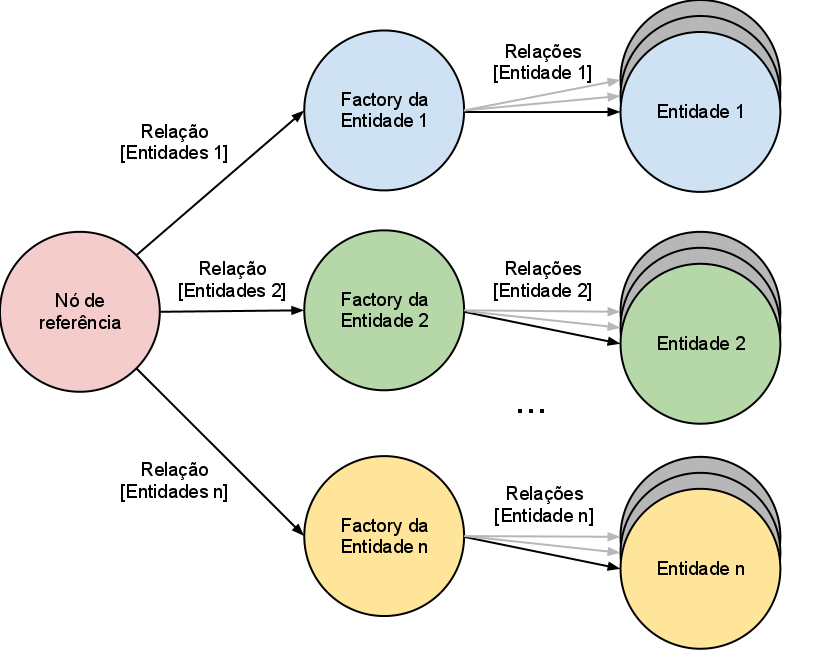
\includegraphics[width=0.7\textwidth]{./imgs/grafoFactory.png}
	\caption[Arquitetura do sistema]{Visão geral da organização das \emph{factories} do grafo.}
	\fonte{Autoria Própria}
	\label{fig:grafoFactory}
\end{figure}

A partir do nó de referência do grafo tem-se relações às \emph{factories} de todas as entidades (relação no formato [Entidades X]), sendo que estas tem relações a cada nó de seu tipo entidade (relação no formato [Entidade X]).
Com estas relações, a \emph{factory} pode ser utilizada para acessar todas as entidades do mesmo tipo, bastando percorrer o grafo.

O uso deste tipo de arquitetura torna o sistema flexível quanto ao SGBD, sendo que se necessária alguma modificação basta atualizar as \emph{factories} de acordo com o novo banco de dados. 
A seguir serão descritas todas as entidades pertencentes ao sistema, bem como a classe responsável pela interface com o banco de dados.

\subsection{Entidades}
As entidades que compõem o \emph{Core}, juntamente com suas \emph{factories}, são representadas através de interfaces e suas respectivas implementações por meio de classes no sistema. 
Desta forma toda entidade é representada no sistema através de duas interfaces e suas respectivas implementações, as quais obedecem o seguinte padrão de nomenclatura e localização (nesse contexto, \texttt{Entidade} consiste em uma representação genérica de qualquer tipo de entidade presente no sistema):
\begin{itemize}
	\item \texttt{Entidade}: interface da entidade do tipo \texttt{Entidade}.
		  Este tipo de representação é localizado no pacote \texttt{com.onibuscerto.core.entities}.
	\item \texttt{EntidadeFactory}: interface referente a \emph{factory} da \texttt{Entidade}.
		  Todas as interfaces de \emph{factories} estão localizadas no pacote \texttt{com.onibuscerto.core.factories} do subprojeto \texttt{onibuscerto-core}.
	\item \texttt{EntidadeImpl}: implementação da interface \texttt{Entidade}.
		  Todos estas implementações estão disponibilizados no pacote \texttt{com.onibuscerto.core}.
	\item \texttt{EntidadeFactoryImpl}: implementação da \emph{factory} da entidade de nome \texttt{Entidade}.
		  Estas implementações estão disponibilizadas no pacote \texttt{com.onibuscerto.core}.
\end{itemize}

Cada entidade do sistema possui suas respectivas propriedades, as quais são armazenadas no próprio nó ou aresta do grafo (dependendo de como a entidade foi armazenada no banco de dados) através de pares chave/valor, sendo estas disponíveis para futuras consultas.

%As interfaces que representam as entidades e suas \emph{factories} pertencem ao pacote \texttt{com.onibuscerto.core.entities} e %\texttt{com.onibuscerto.core.factories}, respectivamente.
%Já as implementações das mesmas estão localizadas no pacote \texttt{com.onibuscerto.core}.

A seguir serão descritos detalhes de implementação das classes que encapsulam as entidades, as quais em conjunto formam o grafo armazenado no banco de dados do sistema.

\subsubsection{Location}
Entidade responsável principalmente por representar pontos através de coordenadas geográficas, bem como suas conexões com outros pontos.
Contém basicamente em quatro atributos: 

\begin{itemize}
	\item \texttt{latitude}: latitude do ponto \emph{Location} em questão.
	\item \texttt{longitude}: longitude do ponto \emph{Location} em questão.
	\item \texttt{outgoingConnections}: coleção de conexões de entrada da \emph{Location}, representadas pela entidade do tipo \emph{Connection} (ver seção 					  \ref{conn}).
	\item \texttt{incomingConnections}: coleção de conexões de saida da \emph{Location}, também representadas pela entidade do tipo \emph{Connection} (ver seção 			  	  \ref{conn}).
\end{itemize}

A \emph{factory} assignada a esta entidade denomina-se \emph{LocationFactory} e, para este tipo de entidade, tem a funcionalidade de criar todas as entidades do tipo \emph{Location}, inclusive  suas extensões, como é o caso da entidade \emph{Stop} descrita na subseção \ref{stop}.

Esta entidade é utilizada principalmente para demarcar os pontos de origem e destino fornecidos pelo usuário que não consistem em uma parada para embarque e desembarque de passageiros.
Esta demarcação é importante para que estes pontos sejam adicionados ao grafo, desta forma contribuindo para um melhor refinamento na busca da rota com tempo de viagem mínimo.

\subsubsection{Stop}
\label{stop}
Uma \emph{Stop} consiste em uma parada de veículos para embarque e desembarque de passageiros.
Como esta também é representada por coordenadas geográficas então optou-se por implementá-la como um caso específico de uma \emph{Location}, ou seja, uma \emph{Stop} herda atributos de \emph{Location}. Desta forma, além dos atributos de \emph{Location}, cada entidade deste tipo possui os seguintes atributos:

\begin{itemize}
	\item \texttt{id}: identifica exclusivamente uma parada ou estação, porém diversos trajetos podem usar a mesma parada.
	\item \texttt{name}: nome de uma parada ou estação.
\end{itemize}

Como uma \emph{Stop} é uma especificação de \emph{Location}, utiliza-se a mesma \emph{LocationFactory}, porém neste caso com as seguintes funcionalidades:
\begin{itemize}
	\item além de criar \emph{Locations}, utiliza-se esta \emph{factory} também para criar entidades \emph{Stop} e adicioná-las a seus respectivos índices no banco 		de dados, com o intuito de facilitar futuras buscas.
	\item retornar todas as \emph{Stops} do sistema em forma de uma coleção, através de simples uma busca no grafo do sistema.
	\item retornar uma determinada \emph{Stop} com base em sua ID utilizando o índice referente a este tipo de entidade.
\end{itemize}

A informação de todas as \emph{Stops} é essencial para o funcionamento do sistema, pois sem as localizações das paradas de veículos é impossível fornecer uma rota entre dois pontos utilizando transporte público.

\subsubsection{Route}

\subsubsection{Trip}

\subsubsection{StopTime}

\subsubsection{Connection}
\label{conn}

\subsection{DatabaseController}


\section{onibuscerto-importer}

\section{onibuscerto-service}

O subprojeto \texttt{onibuscerto-service} é onde encontram-se os Servlets responsáveis por executar consultas na base de dados construída através do \emph{Importer}.
Os Servlets funcionam sob a forma de \emph{web services} e, sendo assim, todas as consultas são feitas pelos clientes através de requisições \sigla{HTTP}{Hypertext Transfer Protocol} do tipo GET ou POST.
As implementações dos Servlets residem no pacote \texttt{com.onibuscerto.service.servlets}.

Atualmente, apenas consultas que determinam a rota com o menor tempo de viagem entre duas coordenadas geográficas estão implementadas.
Estas consultas são de responsabilidade do Servlet implementado na classe \texttt{RouteServlet}.
No início do seu ciclo de vida, este é responsável por obter uma instância da classe \texttt{DatabaseController} do \emph{Core}, a qual será utilizada para acessar o banco de dados e resolver as consultas.
Em seguida, assim como um Servlet comum, este muda para um estado no qual está disponível para atender requisições dos clientes.
Por fim, ao ser destruído, o \texttt{RouteServlet} deve chamar o método \texttt{close} do \texttt{DatabaseController}, com o objetivo de fechar a conexão com o banco de dados.
O ciclo de vida completo de um Servlet é ilustrado na Figura \ref{fig:servletciclo}.

\begin{figure}[!htb]
	\centering
	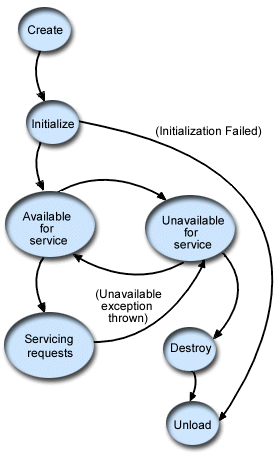
\includegraphics[width=0.4\textwidth]{./imgs/servletciclo.png}
	\caption[Ciclo de vida de um Servlet]{Ciclo de vida de um Servlet}
	\fonte{\citeonline{infocenter}}
	\label{fig:servletciclo}
\end{figure}

Enquanto o \texttt{RouteServlet} está ativo, ou seja, respondendo consultas, este recebe requisições HTTP do tipo POST com os seguintes parâmetros:
\begin{itemize}
	\item \texttt{start.latitude}: latitude do ponto de origem.
	\item \texttt{start.longitude}: longitude do ponto de origem.
	\item \texttt{end.lagitude}: lagitude do ponto de destino.
	\item \texttt{end.longitude}: longitude do ponto de destino.
	\item \texttt{departure}: horário de saída do ponto de origem, uma \emph{string} no formato \texttt{"HH:MM"}.
\end{itemize}

Ao receber estes parâmetros, o \texttt{RouteServlet} executa os seguintes passos:
\begin{enumerate}
	\item Converte as posições geográficas passadas como parâmetros para a consulta através de HTTP POST para objetos da classe \texttt{GlobalPosition}, do subprojeto \texttt{onibuscerto-api}.
	\item Cria nós no banco de dados para representar os nós de origem e destino, através da \texttt{LocationFactory}.
	\item Cria conexões do tipo \texttt{WalkingConnection} entre os recém-criados nós de origem e destino e todas as entidades do tipo \texttt{Stop} do grafo, de forma a representar os trechos que podem ser percorridos a pé pelo usuário.
	\item Executa a consulta no grafo através do método \texttt{getShortestPath} do \texttt{DatabaseController} e recebe o caminho encontrado sob a forma de um objeto do tipo \texttt{Collection<Connection>}.
	\item Converte o resultado da consulta para uma coleção de objetos da classe \texttt{QueryResponseConnection}, do subprojeto \texttt{onibuscerto-api}, ou seja, um objeto do tipo \texttt{Collection<QueryResposeConnection>}.
	\item Serializa o objeto \texttt{Collection<QueryResponseConnection>} para uma \emph{string} no formato \sigla{JSON}{JavaScript Object Notation}, o qual será finalmente enviado para o cliente do usuário.
\end{enumerate}

Tendo o funcionamento do \texttt{RouteServlet} em vista, a aplicação cliente é responsável apenas por enviar uma requisição HTTP POST para o serviço com os parâmetros no formato especificado e, por fim, interpretar os resultados retornados pelo servidor.
Uma pequena aplicação de exemplo que executa consultas no \emph{Service}, escrita em linguagem Python, é apresentada no Apêndice \ref{ape:exemplodeuso}.

\subsection{Cliente \emph{Web}}

Além dos Servlets responsáveis pelo funcionamento do \emph{web service}, o projeto \texttt{onibuscerto-service} é onde também reside o código-fonte do cliente \emph{web}.
Situado no diretório \texttt{src/main/webapp/} deste projeto, o cliente \emph{web} é composto pelos seguintes arquivos:

\begin{itemize}
	\item \texttt{index.html}: estrutura em \sigla{HTML}{Hypertext Markup Language} do \emph{layout} da página que é exibida para os usuários do cliente.
	\item \texttt{style.css}: descrição das folhas de estilo \sigla{CSS}{Cascading Style Sheets} utilizadas para renderizar o \emph{layout} da página.
	\item \texttt{script.js}: código-fonte principal do cliente, em linguagem JavaScript, responsável por todas as funcionalidades e interação do cliente \emph{web} com o service e o usuário.
\end{itemize}

Além destes arquivos, juntamente com a distribuição do cliente \emph{web} estão empacotadas as bibliotecas jQuery e jQuery UI, utilizadas para simplificar o desenvolvimento do \emph{software} em JavaScript.
Estas bibliotecas encontram-se no diretório \texttt{src/main/webapp/js/} do projeto.
As imagens utilizadas no \emph{layout} da página estão presentes no diretório \texttt{src/main/webapp/img/}.

A interface do cliente \emph{web} é composta basicamente por dois elementos: uma barra lateral e a visualização do mapa da região.
Na barra lateral está presente um formulário, através do qual o usuário pode digitar os endereços de origem e destino do caminho e o horário de partida.
Esta mesma barra é atualizada com uma descrição textual do caminho determinado pelo sistema, assim que o usuário inicia a consulta ao clicar no botão de busca.
Além disso, é possível introduzir os endereços de origem e destino clicando com o botão direito do mouse no mapa.
A figura \ref{fig:clienteweb} apresenta a interface do cliente \emph{web} com o resultado de uma consulta.

\begin{figure}[!htb]
	\centering
	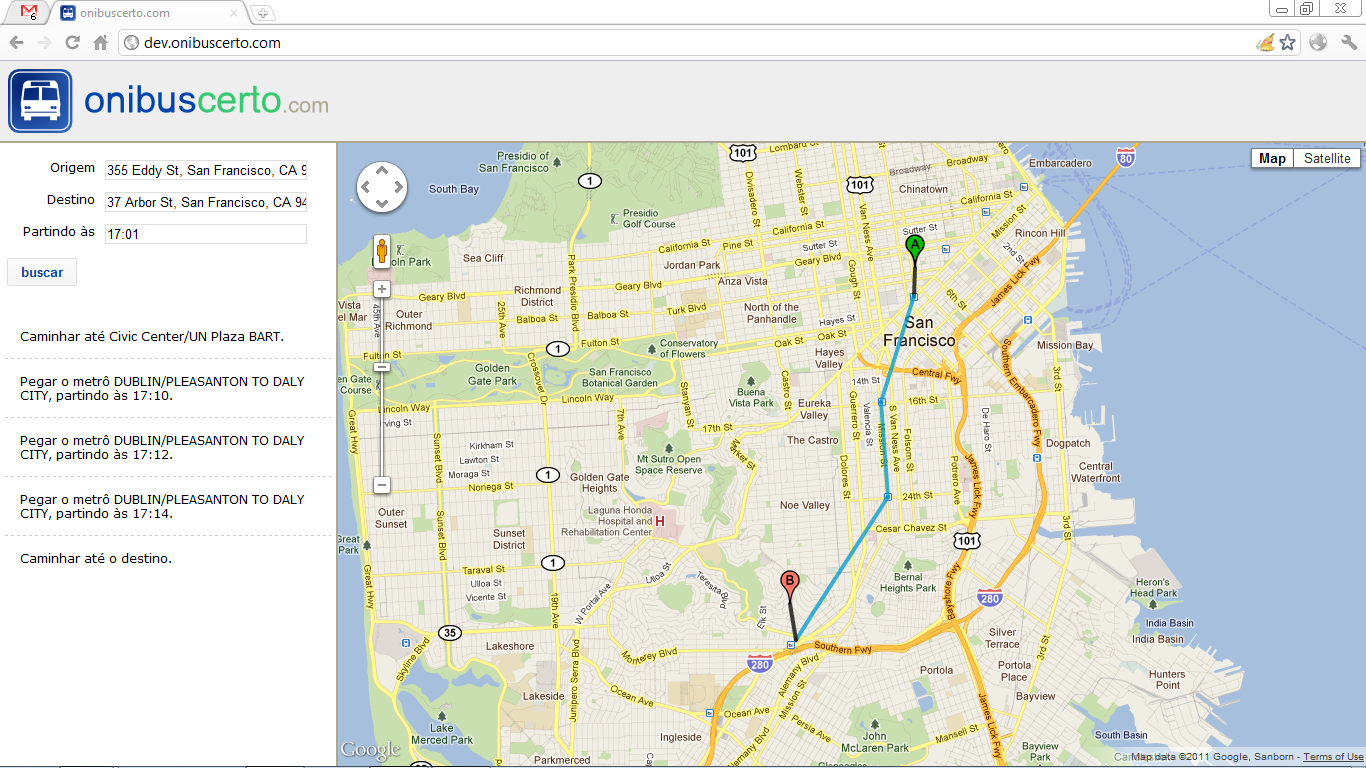
\includegraphics[width=0.9\textwidth]{./imgs/clienteweb.png}
	\caption[Interface do cliente \emph{web}]{Interface do cliente \emph{web}}
	\fonte{Autoria Própria}
	\label{fig:clienteweb}
\end{figure}

A renderização do mapa é feita através da \sigla{API}{Application Programming Interface} do Google Maps \cite{gmapsapi}, a qual permite utilizar, através de chamadas JavaScript, os mapas deste serviço de forma gratuita, contanto que o serviço que faça uso dos mapas também o seja \cite{gmapsterms}.
Esta API também conta com funcionalidades para o desenho de poli-linhas e o posicionamento de marcadores, tornando-se ideal para apresentar os resultados da consulta retornados pelo \emph{web service}.

Para realizar o processo de \emph{geocoding}, ou seja, a conversão de endereços completos como, por exemplo, ``1600 Amphitheatre Parkway, Mountain View, CA'' em coordenadas geográficas como $(37.423021, -122.083739)$, foi utilizada a API de \emph{Geocoding} do Google \cite{geocodingapi}.
De forma semelhante à API do Google Maps, esta API permite realizar este tipo de consulta diretamente através de JavaScript, sendo fornecido um endereço completo e retornando a latitude e longitude do endereço em questão.

O cliente \emph{web} pode ser utilizado simplesmente ao hospedar os arquivos do mesmo em um servidor HTTP.
No entanto, é importante notar que, caso o endereço do \emph{web service} seja diferente da página inicial do cliente \emph{web}, é necessário adaptar o endereço que é feito na requisição do mesmo, no arquivo \texttt{script.js}.
Apesar disso, ao iniciar o servidor de desenvolvimento, o cliente \emph{web} é automaticamente servido através do mesmo.
Maiores detalhes com relação à execução do \emph{software} em um ambiente de desenvolvimento estão disponíveis no Apêndice \ref{ape:guia}.

\section{Considerações}
